\documentclass[
	%a4paper, % Use A4 paper size
	letterpaper, % Use US letter paper size
]{jdf}

\addbibresource{references.bib}

\author{Andrew Myers}
\email{amyers72@gatech.edu}
\title{CS 7646: Project 6 - Indicators and Techinically Optimal Strategy}

\begin{document}
%\lsstyle

\maketitle

\begin{abstract}
	Welcome to Joyner Document Format (JDF) v2.2! JDF is primarily intended to standardize page lengths while ensuring readability. 
	Note that you are required to use JDF for all written assignments, but we will not perform explicit formatting checks. 
	So, while improper formatting may be subject to penalties, you should not worry too much about whether your submission conforms to 
	every minute detail; the most important elements are margins, font, font sizes, and line spacing. Just make a copy of one of the provided templates 
	and replace its contents with your own, using the built-in paragraph styles.\footnote{Here are instructions for 
	\href{https://support.office.com/en-us/article/Video-Using-Styles-in-Word-9db4c0f4-2754-4294-9758-c14a0abd8cfa}{Microsoft Word}, 
	\href{https://support.apple.com/guide/pages/intro-to-paragraph-styles-tanaa39b0aa3/mac}{Apple Pages}, and 
	\href{https://www.bazroberts.com/2016/04/19/google-docs-paragraph-styles-headings/}{Google Docs}.} If you do so, you do not need to verify that the style was followed.
\end{abstract}

\section{Indicators}
\subsection{Simple Moving Average (SMA)}
The Simple Moving Average indicator (SMA) tracks the mean price of an asset over N days. To calculate it over a period of time, we first retrieve the pricing data for the asset.
When we do this, we opt to get data for extra days before the beginning of the specified period so that we can calculate the SMA for the first N days. 
We naively do this by subtracting (N + 30) days from the start date, and use this as the first day of data to retrieve.
Once we have all of the pricing data, we remove non-trading days (NaN) so they do not impact our indicators.
Finally, we can calculate the rolling mean of prices over N days to get the SMA. To make the data easy to use, we can join the data against the date range to readd the NaN values.
For these indicators, we are choosing to leave 'NaN' on non-trading days instead of forward filling. This is to ensure non-trading days do not impact our analysis.

SMA is a useful indicator to track the long-term trends of an asset. It is less sensitive to short-term fluctuations. 
An analyst could hypothesize that over time, prices will revert to the mean. SMA would be a perfect indicator for this strategy.
A simple implementation would be to buy when the price is below 95% * SMA, and sell when the price is above 105% * SMA.

\begin{jdffigure}
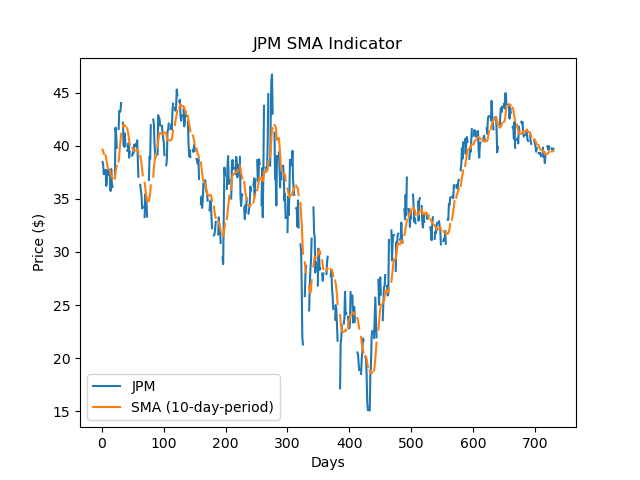
\includegraphics[height=6cm]{Figures/Figure1.png}%
\captionof{figure}{This graph shows the Price and SMA for the asset "JPM" over the period January 1, 2008, to December 31, 2009, with a lookback period of 10 trading days.}
\end{jdffigure}
\textbf{Figure 1} shows the SMA for JPM alongside the price.
These can be used together to visually show longer-term trends in the assets price.


\subsection{Relative Strength Index (RSI)}
The Relative Strength Index (RSI) is an indicator used to measure the speeds and chinges of an asset's price movements. 
It does this by comparing the size of recent gains to recent losses.
It uses a lookback period similar to SMA, so we start by retrieving price data earlier than the start date in the same way as described in 1.1.
Once we have the pricing data, we calculate the pricing difference of each day from the previous day. 
We can then separate the "gains" from the "losses" based on whether that difference was positive or negative.
Once we have the gains and losses, we calculate the averages for each of them over the lookback period N.
Finally, we can calculate the RSI for each day using the formula: RSI = 100 - (100 / (1 + (average gain / average loss))).
A value of 70 or above is generally considered overbought, and a value of 30 or below is generally considered oversold.
Similar to SMA in 1.1, we are choosing to leave 'NaN' on non-trading days instead of forward filling.

RSI can be useful in trading strategies to help identify conditions where the asset is overbought or oversold.
An analyst could use RSI along with SMA to try and identify situations where a new uptrend is beginning for an asset.
To do this, they could buy when the RSI is below 30 (signalling oversold) and price crosses above the SMA.
The opposite would be to sell when the RSI is above 70 (signalling overbought) and price crosses below the SMA.

\begin{jdffigure}
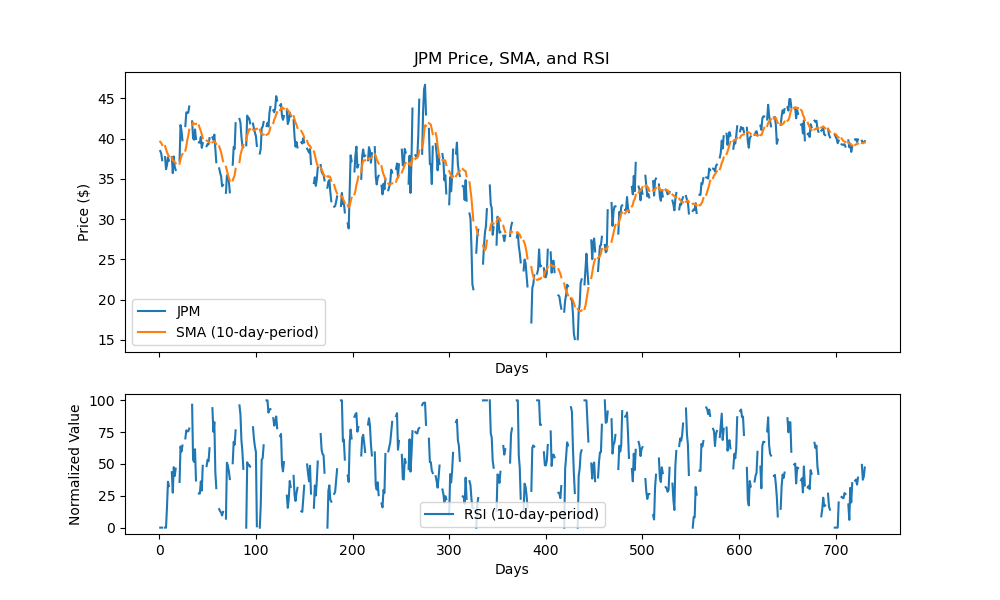
\includegraphics[height=6cm]{Figures/Figure2.png}%
\captionof{figure}{This graph shows the RSI for the asset "JPM" over the period January 1, 2008, to December 31, 2009, with a lookback period of 10 trading days. The Price and SMA are also shown above the RSI.}
\end{jdffigure}
\textbf{Figure 2} shows the RSI for JPM. It is often shown under the price chart, as shown here, with the RSI line oscillating between 0 and 100.
We also included the SMA to demonstrate visually how the analyst could use these indicators together as in the strategy described above.

\subsection{Rate of Change (ROC)}
The Rate of Change (ROC) indicator is used to measure the percentage change in price between the current price and the price N days ago.
It can be used by analysts to measure how quickly the price of an asset is changing.
To calculate the ROC, we first retrieve the pricing data for the asset in the same way as described in 1.1, with N + 30 extra days.
Once we have the data, we can calculate the ROC for each day using the formula: ROC = ((price - price\_N\_periods\_ago) / price\_N\_periods\_ago) * 100.
As we have done with the past indicators, we choose to remove 'NaN' during calculation and add them back in after the calculation is complete.

An analyst could choose to use ROC to signal strong trends in the asset's price. 
They may hypothesize that high ROC signals strong upward momentum, and low ROC signals strong downward momentum.
They could create a strategy that buys the asset when the ROC is above 10%, and sells when the ROC is below 10%.

\begin{jdffigure}
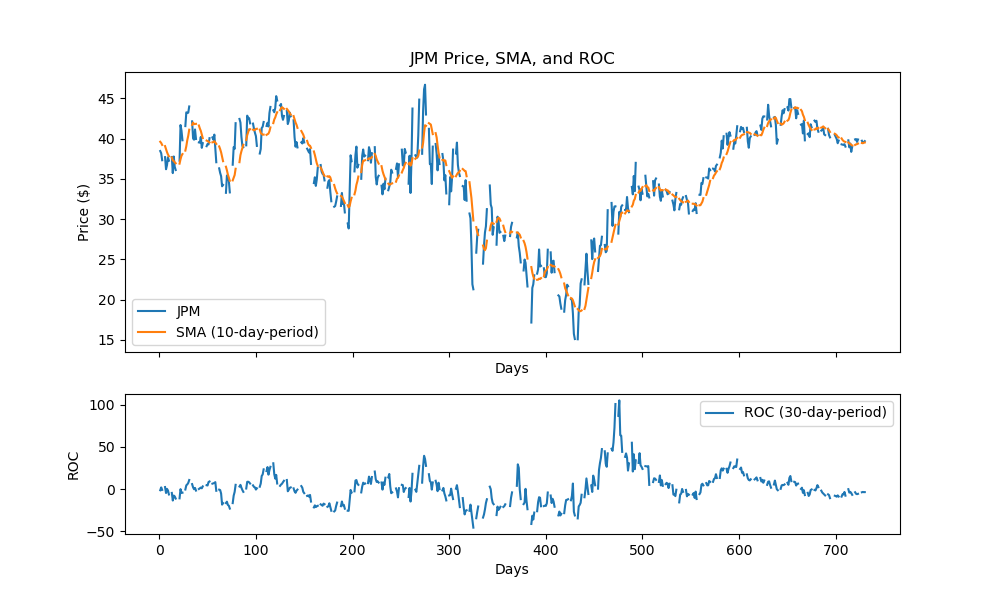
\includegraphics[height=6cm]{Figures/Figure3.png}%
\captionof{figure}{This graph shows the ROC for the asset "JPM" over the period January 1, 2008, to December 31, 2009 with a lookback period of 30 days.}
\end{jdffigure}
\textbf{Figure 3} shows the ROC for JPM. Similarly to RSI, it is often shown under the price chart. Analysts can find trends visually using this graph by watching when the ROC crosses the midpoint 0.

\subsection{Percentage Price Oscillator (PPO)}
The Percentage Price Oscillator (PPO) is a momentum indicator that measures the difference between two moving averages. It is expressed as a percentage of the larger moving average.
To calcualte the PPO, we first need to choose two periods, one long and one short. For this report, we choose to always set the short period to 5 trading days so we can limit the indicator to only one parameter which will be the long period.
We can then calculate the SMA of the asset's price over each of these periods using the SMA indicator from 1.1.
Once we have the two SMAs, we can calculate the PPO using the formula: PPO = 100 * (short\_SMA - long\_SMA) / long\_SMA.

PPO can be used to identify the momentum or trends of an asset's price. A positive PPO indicates that the short-term moving average is above the long-term moving average, which could be a bullish signal.
Alternatively, a negative PPO could signal a downtrend and be a bearish signal. An analyst could use PPO to identify when the momentum of an asset is changing, and use this to inform their trading strategy.
A simple strategy could be to buy when the PPO becomes positive and sell when the PPO becomes negative.

\begin{jdffigure}
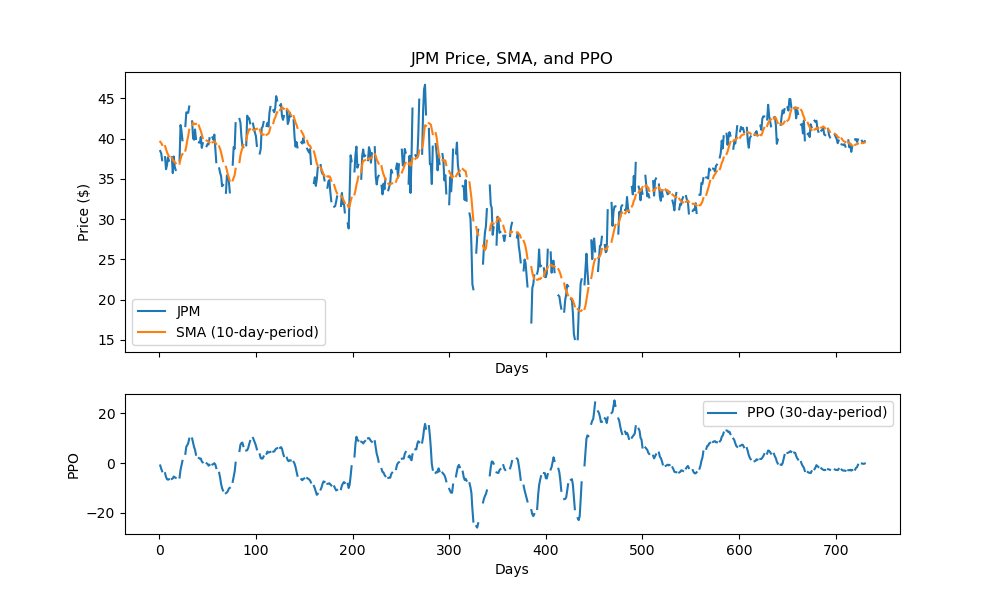
\includegraphics[height=6cm]{Figures/Figure4.png}%{\huge Handgloves}%
\captionof{figure}{This graph shows the PPO for the asset "JPM" over the period January 1, 2008, to December 31, 2009 with a lookback period of 30 days.}
\end{jdffigure}
\textbf{Figure 4} shows the ROC for JPM. Similarly to ROC, it is often shown under the price chart and oscillates around the 0 line.

\subsection{Fast Stochastic Oscillator (\%K)}
The Fast Stochastic Oscillator is a momentum indicator that compares the closing price of an asset to its price range over a specified period.
It is expressed as a percentage called \%K, and can be used to determine where a price is relative to its recent trading range.
We calculate this indicator by first retrieving the pricing data for the asset, again using N + 30 extra days as described in 1.1 to ensure we avoid 'NaN' values caused by the lookback period.
For each day, we then calculate the highest and lowest prices over the past N days.
Finally, we can calculate the \%K for each day using the formula: \%K = 100 * ((price - lowest\_price) / (highest\_price - lowest\_price)).
As with the other indicators, we choose to remove 'NaN' during calculation and add them back in after the calculation is complete.

An analyst could use this indicator as part of a strategy based on the hypothesis that during upward trends, the asset price will tend close relatively high.
Alternatively, during downward trends, the asset price will tend to close relatively low. These trends could be determined using PPO described in 1.4.
They could choose to buy the stock when \%K is below 25\% and PPO is positive with the idea that over time \%K will return to a higher value due to the upward trend.
The opposite would be to sell when \%K is above 75\% and PPO is negative, signalling a downtrend.

\begin{jdffigure}
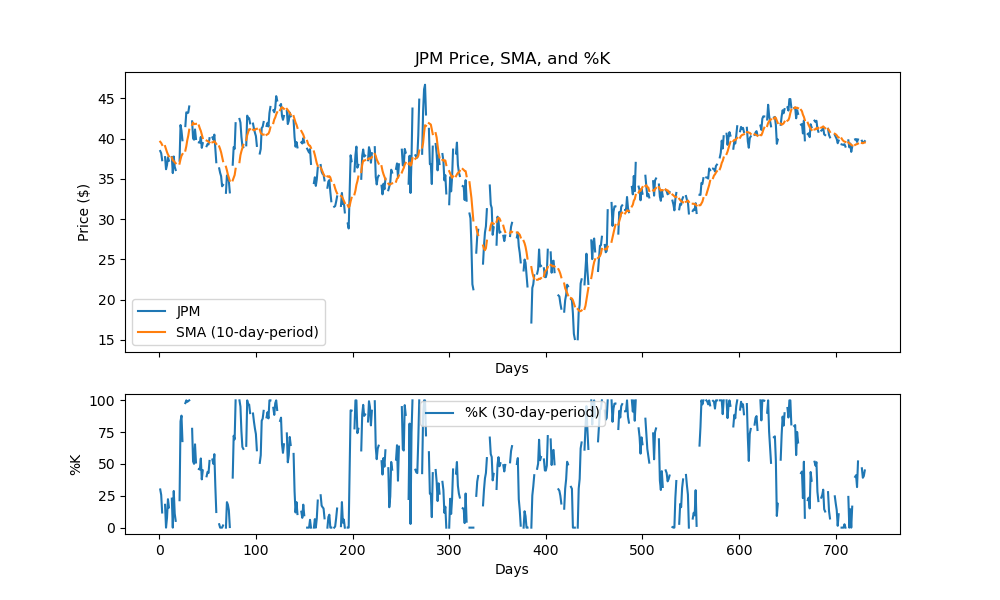
\includegraphics[height=6cm]{Figures/Figure5.png}%{\huge Handgloves}%
\captionof{figure}{This graph shows the PPO for the asset "JPM" over the period January 1, 2008, to December 31, 2009 with a lookback period of 30 days.}
\end{jdffigure}
\textbf{Figure 5} shows the \%K for JPM. It is often shown under the price chart and oscillates between 0\% and 100\%.

\section{Theoretically Optimal Strategy}
\subsection{Description}
In order to provide a benchmark to compare our indicators against, we implement an "optimal" strategy.
This strategy does have the ability to look into the future before choosing to BUY or SELL. 
However, it is constrained in that it's only allowable positions are +1000, 0, and -1000 shares.
We will initiate the benchmark with \$100,000, use "JPM" as the stock symbol, and use the time period January 1, 2008, to December 31, 2009
We also assue commsision and impact are 0, and we are allowing unlimited leverage.

At a high level, the strategy simply buys as many shares as possible when the price will go up, and sells as many shares as possible when the price will go down.
To implement the strategy, we iterate through each day and find that days price as well as the next days price.
If the next days price is higher than the current days price, we move a position of 1000 shares (if not there already).
If the next days price is lower than the current days price, we move a position of -1000 shares (if not there already).
For each of these buy/sell cases, we update our cash total by subtracting the price of the shares bought/sold.
In order to return the results in the form of an order list, each position movement is added to the list as a "BUY" or "SELL" order.

\subsection{Charts}
\begin{jdffigure}
\includegraphics[height=6cm]{Figures/flowchart.png}%{\huge Handgloves}%
\captionof{figure}{This graph shows portfolio value of the Theoretically Optimal Strategy for the asset "JPM" compared to a benchmark of holding 1000 shares. The trades occur over the period January 1, 2008, to December 31, 2009. The portfolio value is calculated by summing the cash and the value of the shares owned.}
\end{jdffigure}
\textbf{Figure 6} shows the results of tradign using the Theoretically Optimal Strategy. 
As expected, the results are much more favorable compared to the benchmark strategy of buying and holding at a position of 1000 for the entire period.

\subsection{Tables}
\begin{jdftable}
\captionof{table}{Theoretically Optimal Strategy results trading JPM.}\label{table:Example}
\small % Reduce font size
\begin{tabular}{@{} L{0.15\linewidth} c S L{0.52\linewidth}}
    \textbf{Strategy} & \textbf{Cumulative Returns} & \textbf{Std. Dev. of Daily Returns} & \textbf{Mean of Daily Returns} \\
    \toprule[0.5pt]
    Benchmark & \$100,000 & 1.618 & \$100,000\\
    \midrule
    Theoretically Optimal & \$100,000 & 1.618 & \$100,000\\
    \midrule
\end{tabular}
\end{jdftable}
    

\end{document}
